%\documentclass[9pt]{scrartcl}
\documentclass[a4paper]{article}
\usepackage[]{amsmath}
\usepackage{tikz}
\usetikzlibrary{positioning}
%\usepackage{helvet}
\usepackage{listings}
\usepackage{geometry}
%\geometry{textheight=\paperheight, noheadfoot, nomarginpar}
\usetikzlibrary{positioning,shapes,shadows}
\renewcommand{\familydefault}{\sfdefault}

\tikzstyle{abstract}=[rectangle, draw=black, fill=gray!20, text centered,  text=black, text width=12.5mm]
\tikzstyle{spacestyle}=[rectangle, draw=black, fill=gray!20, text centered,  text=black, text width=50mm]

\lstset{
        language=python,
        basicstyle=\fontencoding{T1}\ttfamily,
        commentstyle=\color{gray},
        keywordstyle=\color{OliveGreen},
        frame=single,
        backgroundcolor=\color{lightlightgray},
        tabsize=2,
        %deletestring=[d]",
        %escapechar=\%,
        numbers=left,
        showstringspaces=false,
}
\usepackage[explicit]{titlesec} 
\titleformat{\section}{\normalfont\Large\bfseries}{}{0em}{#1}
\titleformat{\subsection}{\normalfont\bfseries}{}{0em}{--#1}

\newcommand{\mykey}[2]{%
\begin{tikzpicture} \node (Item) [abstract, minimum size=12.5mm, align=center]
{\vrule height 12pt depth 8pt width 0pt\textbf{#1} \\\vrule height 6pt depth 8pt width 0pt\parbox{1.25cm}{\centering{\fontsize{6pt}{8pt}\selectfont{#2}}}};%
\end{tikzpicture}}


\begin{document}
\begin{center}
\Large{Diagram}
\end{center}
\noindent%


\section {Architecture diagram}
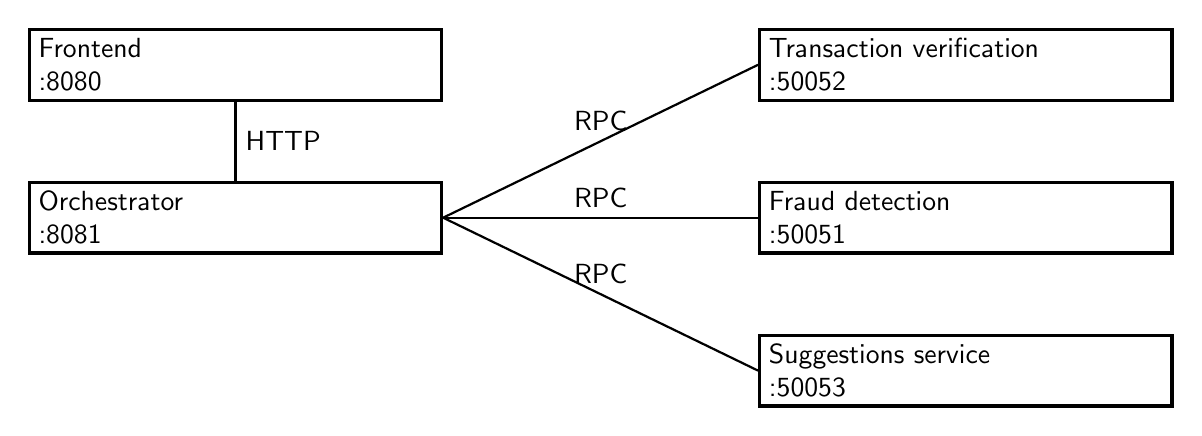
\begin{tikzpicture}

% Frontend
\node [draw,
	minimum width=2cm,
	text width=5cm,
	very thick,
]  (frontend) {
Frontend\\
:8080
};

% Orchestrator
\node [draw,
	minimum width=2cm,
	text width=5cm,
	very thick,
	below = 1cm of frontend
]  (orchestrator) {
Orchestrator\\
:8081
};

% Fraud detection
\node [draw,
	minimum width=2cm,
	text width=5cm,
	very thick,
	right = 4cm of orchestrator
]  (fraud_detection) {
Fraud detection\\
:50051
};

% Transaction verifier
\node [draw,
	minimum width=2cm,
	text width=5cm,
	very thick,
	above = 1cm of fraud_detection
]  (transaction_verification) {
Transaction verification\\
:50052
};

% Suggestions service
\node [draw,
	minimum width=2cm,
	text width=5cm,
	very thick,
	below = 1 cm of fraud_detection
] (suggestions_service) {
Suggestions service\\
:50053
};

% Arrows with text label

\draw[thick] (frontend) -- (orchestrator) node[midway, right] {HTTP};
\draw[thick] (orchestrator.east) -- (fraud_detection.west) node[midway, above] {RPC};
\draw[thick] (orchestrator.east) -- (transaction_verification.west) node[midway, above] {RPC};
\draw[thick] (orchestrator.east) -- (suggestions_service.west) node[midway, above] {RPC};

\end{tikzpicture}


\end{document}